\documentclass[]{article}
\usepackage{lmodern}
\usepackage{amssymb,amsmath}
\usepackage{ifxetex,ifluatex}
\usepackage{fixltx2e} % provides \textsubscript
\ifnum 0\ifxetex 1\fi\ifluatex 1\fi=0 % if pdftex
  \usepackage[T1]{fontenc}
  \usepackage[utf8]{inputenc}
\else % if luatex or xelatex
  \ifxetex
    \usepackage{mathspec}
  \else
    \usepackage{fontspec}
  \fi
  \defaultfontfeatures{Ligatures=TeX,Scale=MatchLowercase}
\fi
% use upquote if available, for straight quotes in verbatim environments
\IfFileExists{upquote.sty}{\usepackage{upquote}}{}
% use microtype if available
\IfFileExists{microtype.sty}{%
\usepackage[]{microtype}
\UseMicrotypeSet[protrusion]{basicmath} % disable protrusion for tt fonts
}{}
\PassOptionsToPackage{hyphens}{url} % url is loaded by hyperref
\usepackage[unicode=true]{hyperref}
\hypersetup{
            pdfborder={0 0 0},
            breaklinks=true}
\urlstyle{same}  % don't use monospace font for urls
\usepackage{graphicx,grffile}
\makeatletter
\def\maxwidth{\ifdim\Gin@nat@width>\linewidth\linewidth\else\Gin@nat@width\fi}
\def\maxheight{\ifdim\Gin@nat@height>\textheight\textheight\else\Gin@nat@height\fi}
\makeatother
% Scale images if necessary, so that they will not overflow the page
% margins by default, and it is still possible to overwrite the defaults
% using explicit options in \includegraphics[width, height, ...]{}
\setkeys{Gin}{width=\maxwidth,height=\maxheight,keepaspectratio}
\IfFileExists{parskip.sty}{%
\usepackage{parskip}
}{% else
\setlength{\parindent}{0pt}
\setlength{\parskip}{6pt plus 2pt minus 1pt}
}
\setlength{\emergencystretch}{3em}  % prevent overfull lines
\providecommand{\tightlist}{%
  \setlength{\itemsep}{0pt}\setlength{\parskip}{0pt}}
\setcounter{secnumdepth}{0}
% Redefines (sub)paragraphs to behave more like sections
\ifx\paragraph\undefined\else
\let\oldparagraph\paragraph
\renewcommand{\paragraph}[1]{\oldparagraph{#1}\mbox{}}
\fi
\ifx\subparagraph\undefined\else
\let\oldsubparagraph\subparagraph
\renewcommand{\subparagraph}[1]{\oldsubparagraph{#1}\mbox{}}
\fi

% set default figure placement to htbp
\makeatletter
\def\fps@figure{htbp}
\makeatother


\date{}

\begin{document}

\section{Rapport d'activité 2020}\label{rapport-dactivituxe9-2020}

\subsection{GDR-CNRS2105 Tresses et topologie de basse
dimension}\label{gdr-cnrs2105-tresses-et-topologie-de-basse-dimension}

\subsection{Contexte}\label{contexte}

L'activité principale du GdR est la promotion et le financement des
conférences organisées par les membres. Le fonctionnement du GdR a été
fortement perturbé par les circonstances sanitaires exceptionnelles en 2020. Au
mois de janvier on avait prévu de participer au financement de sept
conférences mais finalement le bilan est assez maigre :

\begin{itemize}
\tightlist
\item
  une s'est déroulée dans les conditions normales
\item
  une deuxième en distanciel avec les exposés en vidéo
\item
  une troisième a eu lieu en présentiel mais les organisateurs ont dû
  faire face à des problèmes non négligeables.
\end{itemize}

La liste gdrtresses@listes.math.cnrs.fr s'est avérée très utile pour
diffuser les informations concernant l'évolution de status de ces évènements rapidement

\subsubsection{Séminaires virtuels}\label{suxe9minaires-virtuels}

La liste de diffusion a également servi à faire la publicité pour divers
séminaires virtuels :

\begin{itemize}
\tightlist
\item
  Le séminaire virtuel francophone Groupes et Géométrie
\item
  Le séminaire de topologie LAGA/IMJ-PRG
\item
  Geometry and Topology Online (Université de Warwick, UK)
\end{itemize}

\subsubsection{Liste de conférences
prévues}\label{liste-de-confuxe9rences-pruxe9vues}

\begin{itemize}
\tightlist
\item
  WinterBraids X, Pise
\item
  Journées Franco Japonaises, Grenoble
\item
  Artin Groups, CAT(0) Geometry and Related Topics, CIRM
\item
  Conférence internationale à la mémoire de Patrick Dehornoy, Caen
\item
  Teichmüller Theory: Classical, Higher, Super and Quantum, CIRM
\item
  Complex Hyperbolic Geometry and Related Topics, CIRM
\item
  Journées ARA, l'ENSL
\end{itemize}

\subsubsection{Liste de conférences qui ont eu lieu}\label{liste-de-confuxe9rences-pruxe9vues2}

\begin{itemize}
\tightlist
\item
  WinterBraids X, Pise : r-à-s
\item
  Artin Groups, CAT(0) Geometry and Related Topics, CIRM 
  : 0 présents jusqu'à 80 connectés par video.
\item
  Teichmüller Theory: Classical, Higher, Super and Quantum, CIRM
    : 20 présents et jusqu'à 65 connectés par video.
Peu de participants ont pu venir de l’étranger (3 d’Allemagne, et aucun extra-européen, car les frontières étaient fermées).
\end{itemize}

On note que l'équipe du CIRM a fait un gros effort pour mettre en place des solutions de
diffusion des exposés.


\subsubsection{Credits remontés à
l'INSMI}\label{credits-remontuxe9s-uxe0-linsmi}

Suite à la demande de l'INSMI  et compte tenu d'annulations de conferences
évoquées ci-dessus, nous avons rendu 8500 euros au CNRS le
23/9/2020.

\subsection{Production scientifique}\label{production-scientifique}

Les actes de WinterBraids sont publiés
http://www.cedram.org/spip.php?article228\&lang=en

\subsection{Bilan financier}\label{bilan-financiuxe8re}

Le solde au 1/11/2020 est de 383 euros - vu les contraintes sur les
déplacements et les réunions on sera obligé de remonter ces credits à la fin l'année.

\begin{figure*}
\centering
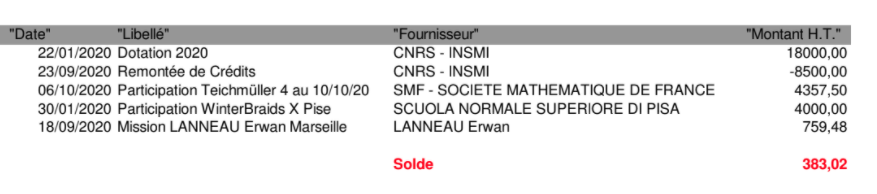
\includegraphics{./budget_tresses.png}
\caption{Résumé des attributions 2020.}
\end{figure*}

\subsection{Perspectives pour 2021}\label{perspectifs-pour-2021}

Étant donné l'évolution de la pandémie l'activité du GdR risque d'être
fortement perturbée en 2021 également. Les organisateurs ont déjà eu à déplacer la  prochaine edition de Winterbraids du mois de février à la rentrée 2021 mais les conferences avec une
participation internationale auront lieu très probablement en
distanciel.

Il n'est pas impossible donc que le GdR n'arrive pas à dépenser les attributions
conformément aux échéances prévues par l'INSMI en 2021.


\end{document}
